\documentclass[tikz,border=10pt]{standalone}
\begin{document}
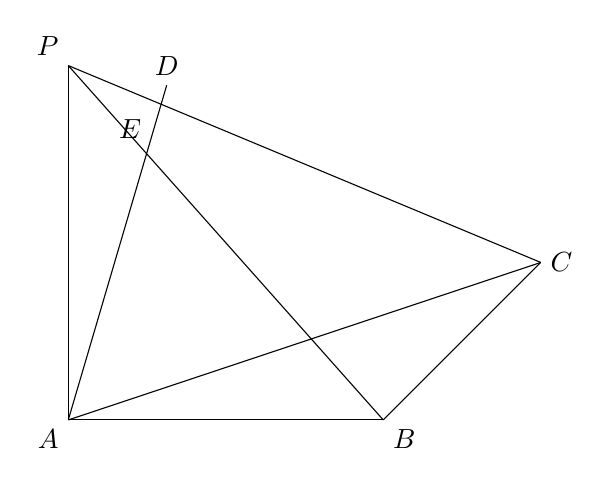
\begin{tikzpicture}[scale=1]
\coordinate (A) at (0,0);
\coordinate (B) at (4,0);
\coordinate (C) at (6,2);
\coordinate (P) at (0,4.5);
\coordinate (D) at (1.25,4.25);
\coordinate (E) at (1.05,3.7);

\draw (A) -- (P);
\draw (P) -- (C);
\draw (P) -- (B);
\draw (A) -- (B);
\draw (B) -- (C);
\draw (A) -- (C);
\draw (A) -- (D);

\node[above left] at (P) {$P$};
\node[above] at (D) {$D$};
\node[left] at (E) {$E$};
\node[below left] at (A) {$A$};
\node[below right] at (B) {$B$};
\node[right] at (C) {$C$};
\end{tikzpicture}
\end{document}
